\section{Interactive LTS synthesis from MSC collections\label{section:lts-induction-from-mscs}}

This section introduces QSM, a Query driven State-Merging synthesis technique. QSM specification is as follows:

\begin{quote}
\underline{Given}
\begin{itemize}
\item A consistent MSC collection showing typical examples and counterexamples of system behaviors:
\begin{align*}Sc = (S^+,S^-)\end{align*}
\item An \emph{oracle} correctly classifying system traces as positive or negative examples of desired system behaviors
\end{itemize}
\underline{Synthesize}~a LTS capturing system behaviors,
\begin{align*}System\end{align*}
\underline{Such that}
\begin{itemize}
\item $Sc$ is correctly extended with the answers to scenario questions by the oracle, and
\item \emph{System} is consistent with the extended scenario collection.
\end{itemize}
\end{quote}

The specification of QSM is similar to the synthesis problem statement in Section~\ref{subsection:inductive-synthesis-statement}. The main differences are related to the presence of the oracle and the fact that the decomposition step is not implemented by QSM itself. Moreover, remember from Section~\ref{subsection:background-scenario-consistency} that requiring the consistency of the input scenario collection amounts to require all scenarios to start in the same system state.

%\begin{itemize}
%\item QSM requires the scenario collection to be consistent. Remember from Section~\ref{subsection:background-scenario-consistency} that this amount to require all scenarios to start in the same system state.
%\item Unlike RPNI, QSM relies on the presence of on oracle. The latter is required to \emph{correctly} classify generated scenario questions, also called \emph{membership queries}. In other words, QSM does not support classification errors. The generation of scenario questions will be detailed in Section~\ref{QSM:query}.
%\item QSM guarantees that the synthesized system LTS and the scenario collection, extended with the classified scenarios, are consistent. Provided preconditions are met, this entails the consistency of the extended collection itself.
%\item Requiring the consistency of the synthesized system LTS with scenarios is weaker than requiring this on the composed system $\agentscomposed$.
%\end{itemize}

Algorithm~\ref{QSM} gives the pseudo-code of the \textsc{QSM} algorithm; RPNI can be seen as a particular instance without the inner-most while loop. Roughly, the induction process starts by constructing an initial LTS covering all positive scenarios only. The LTS is then successively generalized under the control of the available negative scenarios and newly generated scenarios classified by the end-user. This generalization is carried out by successively merging well-selected state pairs from the initial LTS. The process is such that, at any step, the current LTS is consistent with all positive scenarios and all negative ones, including the interactively classified ones. This process terminates when no state pairs can still be considered for merging.

In the sequel, two states will be said compatible for merging (resp. incompatible) if the quotient LTS which results from their merging is consistent (resp. inconsistent) with the current scenario collection.

\begin{algorithm}
{
$A \leftarrow $ {\tt Initialize($Sc$)}\\
\While{$(q,q') \leftarrow $ {\tt ChooseStatePair($A$)}}{
$A_{new} \leftarrow$ {\tt Merge$(A,q,q')$}\\
\If{{\tt Consistent$(A_{new},Sc)$}}{
 \While{$Query \leftarrow $ {\tt GenerateQuery($A,A_{new}$)}}{
   \If{{\tt CheckWithEndUser($Query$)}}{
     $Sc \leftarrow (S_+ \cup \{Query\},~S_-)$
   }\Else{
     $Sc \leftarrow (S_+,~S_- \cup \{Query\})$\\
     \Return{\textsc{QSM}$(Sc)$}
   }
 }
 $A \leftarrow A_{new}$
}
}
\Return{$A,~Sc$}}
\vspace{0.2cm}
\caption{\textsc{QSM}: interactive LTS synthesis based on an input scenario sample and scenario queries\label{QSM}}
\end{algorithm}

In Algorithm \ref{QSM}, the \texttt{Initialize} function returns an initial candidate LTS built from the scenario collection. This function computes $\mathcal{L}^+(Sc)$, the set of positive scenario traces, according to the trace semantics defined in Chapter~\ref{chapter:framework}. Those traces are captured through a PTA; as the positive sample is prefix-closed, this PTA has all accepting states.

Next, pairs of states are iteratively chosen from the current solution according to the \texttt{ChooseStatePair} function\footnote{The assignment in the corresponding \textbf{while} loop is assumed to be \textit{true} whenever a valid state pairs is returned by \texttt{ChooseStatePairs}. When no more state pairs are considered for merging, \texttt{ChooseStatePairs} returns \textit{(nil,nil)} and the assignment is evaluated to \textit{false.} This abuse of notation in the pseudo-code allows to keep it more concise. A similar remark also applies to the inner \textbf{while} loop of the \textsc{QSM} algorithm.}. The quotient automaton obtained by merging such states, and possibly some additional states, is computed by the \texttt{Merge} function. The consistency of this quotient automaton is then checked by the \texttt{Consistent} function using available negative scenarios in the collection. The various functions are more precisely specified hereafter.

When consistent, new scenarios are generated through the \texttt{GenerateQuery} function. These scenarios are submitted to the end-user for classification (see Section~\ref{QSM:query}). The scenario collection is then refined with these scenarios, according to their classification. If all generated scenarios are classified as positive, the quotient automaton becomes the current candidate solution. The process is iterated until no more pair of states can be considered for merging. When a generated scenario is classified as negative, the algorithm is recursively called on the extended scenario collection.

Section~\ref{QSM:merging} describes the general process of merging compatible state pairs while Section~\ref{QSM:query} focuses on the generation of queries submitted to the end-user. Section~\ref{BlueFringe} discusses an optimization of the search order implemented in \texttt{ChooseStatePair} known as the the Blue-Fringe strategy~\cite{Lang:1998}.

\subsection{Merging compatible state pairs\label{QSM:merging}}

The various functions that control how merging is performed from an initial automaton are specified hereafter. 

\begin{description}

\item[Initialize] The \texttt{Initialize} function returns the prefix tree acceptor built for $\mathcal{L}^+(S)$. Remember that this set includes traces from both the positive scenarios and the preconditions of the negative ones. The PTA built from the initial scenario collection in Figure~\ref{Fig:init:scen} is shown on top of Figure~\ref{Fig:algo:steps}. For simplicity, these scenarios define a total order on their events; in other words, they admit one linearization only (see Section~\ref{section:background-scenarios}). 

\begin{figure}
\centering
\scalebox{.56}{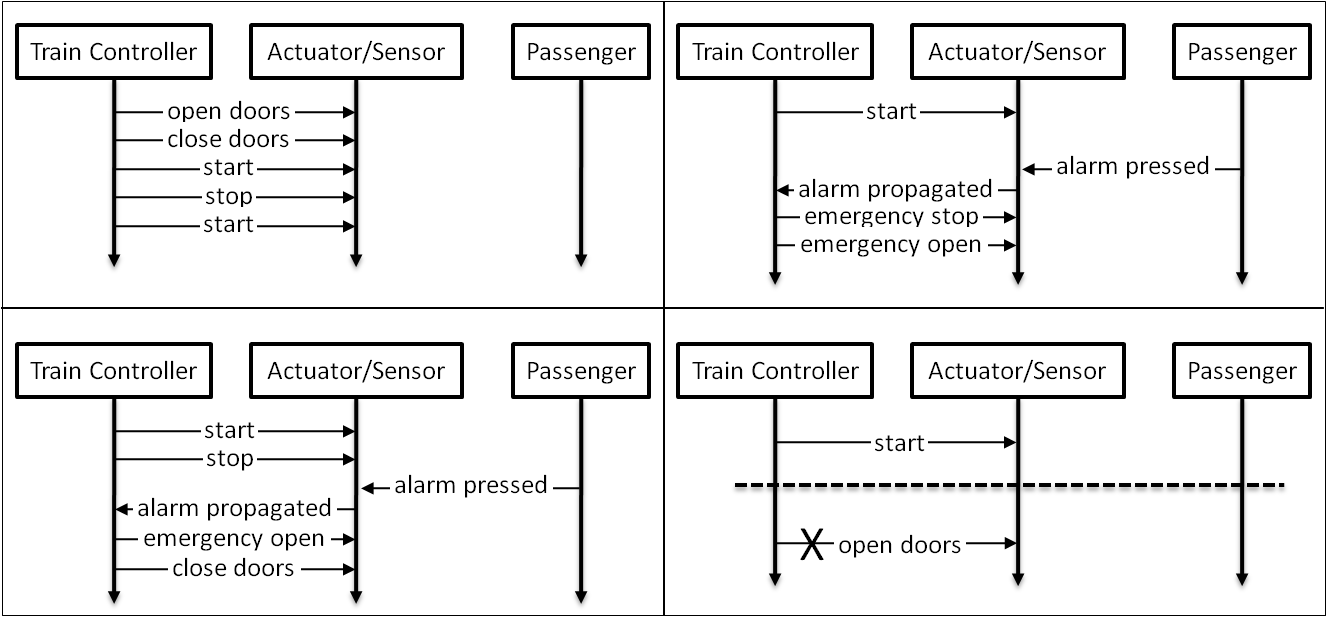
\includegraphics[trim=3mm 3mm 3mm 3mm, clip]{src/4-inductive/images/four-initial-scenarios}}
\caption{Initial positive and negative scenarios for a train system\label{Fig:init:scen}.}
\end{figure}

\item[ChooseStatePair] The candidate solution has to be refined by merging well-selected state pairs. The \texttt{ChooseStatePair} function determines what pairs to consider. It relies on the standard order on strings. Each state of the PTA can be labeled by its unique prefix from the initial state. Since prefixes can be sorted according to that order, the states can be ranked accordingly. For example, the PTA states in Fig.~\ref{Fig:algo:steps} are labeled by their rank according to this order. The algorithm considers states $q$ of the PTA in increasing order. The state pairs considered for merging only involve such state $q$ and any state $q'$ of lower rank. The $q'$ states are considered in increasing order as well. This particular ordering is specific to the original RPNI algorithm.

\item[Merge] The \texttt{Merge} function merges the two selected states $(q, q')$ in order to compute a quotient automaton, thereby generalizing the current set of positive behaviors. 

In the example of Fig.~\ref{Fig:algo:steps}, we assume that states 0, 1, and 2 were previously determined not to be compatible for merging. This information typically comes from negative scenarios initially submitted or generated scenarios that were rejected by the user. 

Merging a candidate state pair may produce a non-deterministic LTS. For example, after having merged $q = 3$ and $q' = 0$ in the upper part of Fig.~\ref{Fig:algo:steps}, two transitions labeled \texttt{start} from state 0 lead to states 2 and 6, respectively. In such case, the \texttt{Merge} function will merge states 2 and 6 and, recursively, any further pair of states that introduces non-determinism. 

This recursive operation of removing non-determinism will be called \textsl{merging for determinization}. This operation guarantees that the current solution at any step is deterministic. As a result, it produces an automaton which may accept a more general language than the one it starts from. Therefore, it is not equivalent to the standard algorithm for transforming a non-deterministic automaton into a deterministic one accepting the same language~\cite{Hopcroft:1979}. Notably, the time complexity of merging for determinization is a \emph{linear} function of the number of states of the automaton it starts from. In contrast, standard determinization is exponential in the worst case. Furthermore, the resulting automaton is still part of the same inductive search space (see Section~\ref{subsection:gi-background-search-space}). 

\begin{figure}[H]
\centering
\scalebox{.75}{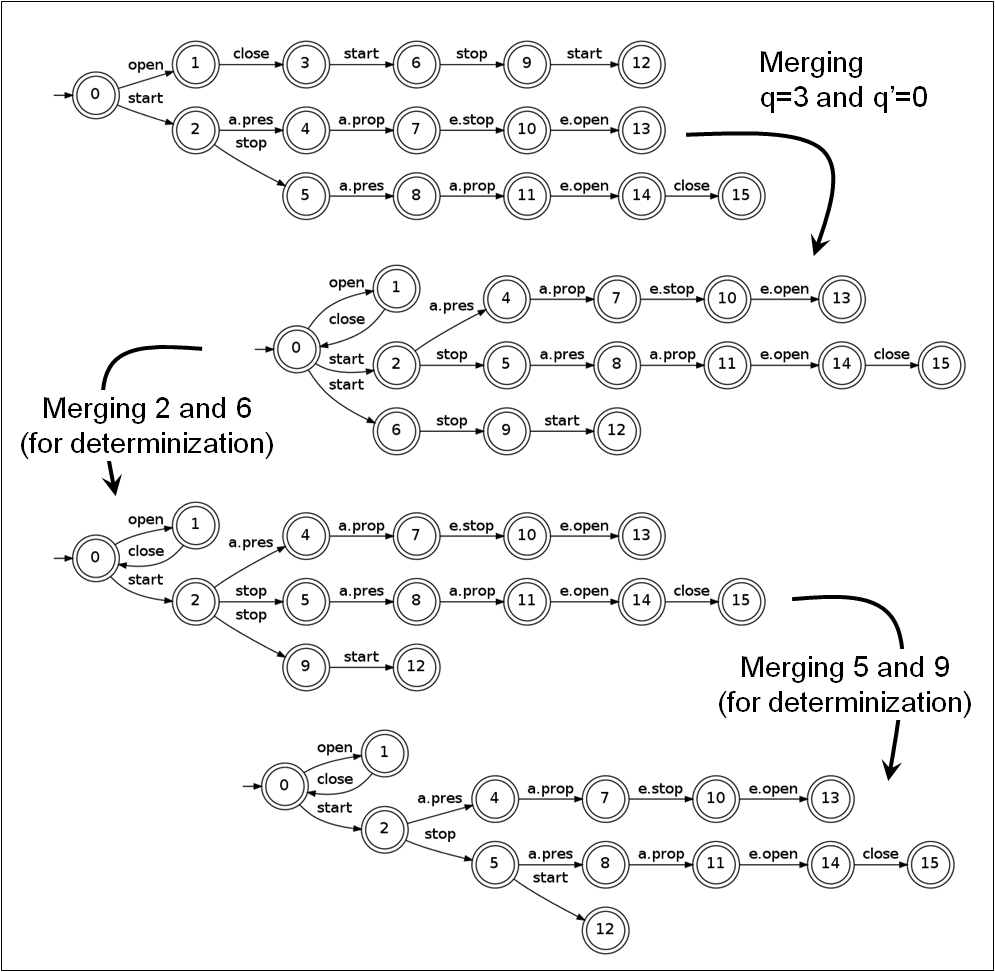
\includegraphics[trim=3mm 3mm 3mm 3mm, clip]{src/4-inductive/images/algo-steps}}
\caption{Induction step of the \textsc{QSM} algorithm\label{Fig:algo:steps}.}
\end{figure}

When two states are merged, the rank of the resulting state is defined as the lowest rank of the pair; in particular, the rank of the merged state when merging $q$ and $q'$ is defined as the rank of $q'$ by construction. If no compatible merging can be found between $q$ and any of its predecessor states according to string ordering, state $q$ is said to be \textsl{consolidated}. In the example, states 0, 1, and 2 are consolidated.

\item[Consistent] The \texttt{Consistent} function checks whether the automaton $A_{new}$ correctly rejects all negative scenarios. As seen in Algorithm~\ref{QSM}, the quotient automaton is discarded by \textsc{QSM} when it is detected not to be consistent.

\end{description}

\subsection{Generating queries submitted to the end-user\label{QSM:query}}

This section describes how queries are generated in the \textsc{QSM} algorithm and how the end-user answers are processed.

\begin{description}

\item[GenerateQuery] When an intermediate solution is consistent with the available scenarios, new scenarios are generated for classification by the end-user as positive or negative. The aim is to avoid overgeneralization by enriching the possibly limited collection of initial scenarios. The notion of characteristic sample drives the identification of which new scenarios should be generated as queries. 

As we saw in Section~\ref{subsection:gi-background-rpni}, a sample is characteristic of a regular language $L$ if it contains enough positive and negative information. On the one hand, the required positive information is the set of short prefixes $Sp(L)$ which form the shortest histories leading to each state of the canonical automaton $A(L)$. This positive information must also include all elements of the kernel $N(L)$; indeed they represent all system transitions, that is, all shortest histories followed by any admissible event. If such positive information is available, $A(L)$ can always be derived from the PTA by an appropriate set of merging operations. On the other hand, the negative traces provide the necessary information to make incompatible the merging of states that should be kept distinct. A negative trace which would exclude the merging of a state pair $(q, q')$ can simply be made of the shortest history leading to $q'$ followed by any continuation from state $q$, as detailed below.

Consider the current solution of our induction algorithm when a pair of states $(q, q')$ is selected for merging (line 5 in Algorithm \ref{QSM}). By construction, $q'$ is always a consolidated state at this step of the algorithm; that is, $q'$ is considered to be in $Sp(L)$. State $q$ is always both the root of a tree and the child of a consolidated state. In other words, $q$ is situated at one symbol of a consolidated state -- that is, $q$ is considered to be in $N(L)$. States $q$ and $q'$ are compatible according to the available negative scenarios; they would be merged by the standard RPNI algorithm. 

The QSM extension will first confirm or infirm the compatibility of $q$ and $q'$ by generating scenarios to be classified by the end-user. The generated scenarios are constructed as follows.

\begin{figure}
\centering
\scalebox{.75}{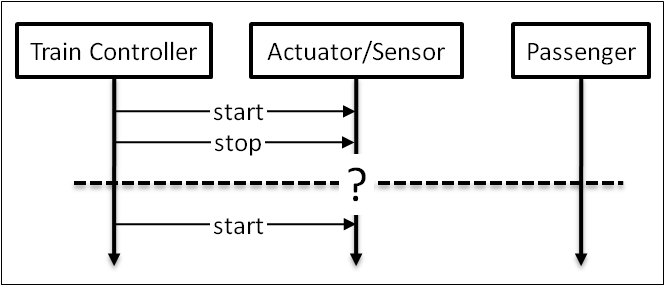
\includegraphics[trim=3mm 3mm 3mm 3mm, clip]{src/4-inductive/images/scenario-question}}
\caption{A new scenario to be classified by the end-user\label{Fig:generated:question}.}
\end{figure}

Let $A$ denote the current solution, $L(A)$ the language generated by $A$, and $A_{new}$ the quotient automaton computed by the \texttt{Merge} function at some given step. Let $x \in Sp(L)$ and $y \in N(L)$ denote the short prefixes of $q'$ and $q$ in A, respectively. Let $u \in L(A)/y$ denote a suffix of $q$ in $A$. 

A generated scenario is built from a system trace $xu$ such that $xu \in L(A_{new})\setminus L(A)$. It can be further decomposed as $xvw$ such that $xv \in L(A)$. The trace $xu$ is thus constructed as the short prefix of $q'$ concatenated with a suffix of $q$ in the current solution, provided the entire behavior is not yet accepted by $A$. 

Such system trace can be converted in a MSC using the structural information provided by a context diagram \cite{Jackson:1995}. The scenario is made of two parts: the first part $xv$ is an already accepted behavior whereas the second part $w$ provides a continuation to be checked for acceptance by the end-user. When submitted to the end-user, the generated scenario can always be rephrased as a question: after having executed the first episode ($xv$), can the system continue with the second episode ($w$)? 

Consider the example in Fig.~\ref{Fig:algo:steps} with selected state pair $q=3, q'=0$. As $q'$ is the root of the PTA, its short prefix is the empty trace $\lambda$. The suffixes of $q$ here yield a simple generated question (see Fig.~\ref{Fig:generated:question}), which can be rephrased as follows: \emph{when having started and stopped the train, can the controller restart it?} As we can see, the first episode of this scenario in Fig.~\ref{Fig:algo:steps} is already accepted by $A$ whereas the entire behavior is accepted in $A_{new}$.

\item[CheckWithEndUser] Whenever a new scenario is generated, it is submitted as a query to the end-user. If the end-user classifies the $Query$ as positive, it is added to the collection of positive scenarios. This addition extends the search space as it extends $S^+$ and consequently the PTA. However, this extension is implicit as the new solution $A_{new}$ is, by construction, also a quotient automaton of this extended PTA. When the $Query$ is classified as negative, the induction process is recursively started on the extended scenario collection.

\end{description}

The QSM algorithm has a polynomial time complexity in the size of the learning sample $\mathcal{L}^+(Sc)$, see \cite{Dupont:2008}. 

When the algorithm receives a characteristic sample in the initial scenario collection, no additional scenario can be classified as negative. As a consequence, QSM will not be called recursively anymore; it stops by returning the target model. 

Chapter~\ref{chapter:evaluation} will detail an experimental study of the actual sample size required to observe the convergence of \textsc{QSM} and the number of queries submitted to the end-user.

\subsection{Reducing the number of queries: the blue-fringe optimization\label{BlueFringe}}

The order in which states are considered for merging by the \texttt{ChooseStatePair} function in Section~\ref{QSM:merging} follows from the implicit assumption that the current sample is characteristic. Two states are considered compatible for merging if there is no suffix to distinguish among them. This can lead to a significant number of scenarios being generated to the end-user in case the initial sample is sparse and actually not characteristic for the target system LTS. 

To overcome this problem, an optimized strategy known as Blue-Fringe \cite{Lang:1998} can be used. The difference lies in the way state pairs are considered for merging. The general idea is to detect incompatible state pairs early and, subsequently, to first consider state pairs for which compatibility has the highest chance to be confirmed by the user through positive classification. The resulting ``please confirm'' interaction may also appear more appealing to the user.

\begin{figure}
\centering
\scalebox{.55}{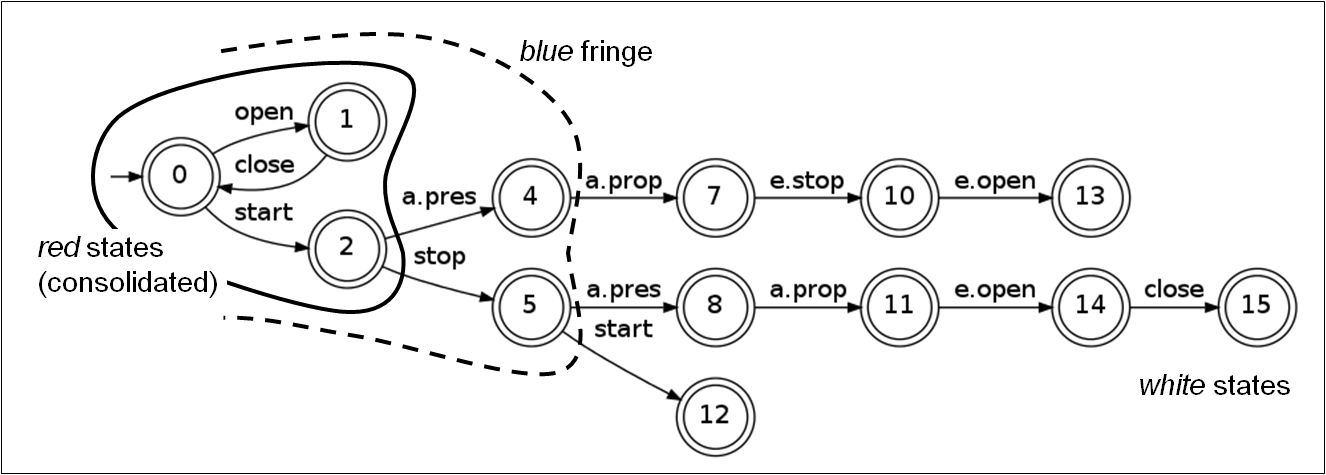
\includegraphics[trim=3mm 3mm 3mm 3mm, clip]{src/4-inductive/images/blue-fringe}}
\caption{Consolidated states (red) and states on the fringe (blue) in a temporary solution\label{Fig:BlueFringe}.}
\end{figure}

Fig.~\ref{Fig:BlueFringe} gives a typical example of a temporary solution produced by the original algorithm. Three state classes can be distinguished in this LTS. The so-called ``red'' states are the consolidated ones (0, 1 and 2 in this example). Outgoing transitions from red states lead to the ``blue'' states unless the latter have already been labeled as red. Blue states form the blue fringe (4 and 5 in this case). All other states are called the ``white'' states. 

The original \texttt{ChooseStatePair} function in Section~\ref{QSM:merging} considers the lowest-rank blue state first (state 4 here) for merge with the lowest-rank red state (0). When this choice leads to a compatible quotient automaton, scenarios are generated to the end-user for classiciation -- in this case, a scenario equivalent to the trace \artifact{<alarm propagated, emergency stop, emergency open>}. 

The above strategy may lead to multiple queries being generated to avoid overgeneralization. Moreover, such queries may be non-intuitive for the user, \textit{e.g.} the \artifact{alarm propagated} event is sent to the train controller without having been fired by the \artifact{alarm pressed} event to the sensor.

To select a state pair for merging, the Blue-Fringe strategy evaluates all (red, blue) state pairs first. The \texttt{ChooseStatePair} function will now call the \texttt{Merge} and \texttt{Compatible} functions before selecting the next state pair. If a blue state is found to be incompatible with all current red states, it is immediately promoted to red; the blue fringe is updated accordingly and the process of evaluating all (red, blue) pairs is iterated. When no blue state is found to be incompatible with red states, the most compatible (red, blue) pair is selected for merging. This is dictated by a scoring mechanism implemented in the \texttt{Compatible} function (see below).

When implementing the Blue-Fringe strategy, it appears convenient to adapt \texttt{Initialize} so as to build an \emph{augmented} prefix tree acceptor. Such PTA captures the negative traces in $\mathcal{L}^-(Sc)$ in addition to the positive traces in $\mathcal{L}^+(Sc)$. States reached by a negative trace are tagged as error states; they are depicted in black, as in Fig. \ref{figure:augmented-pta}. 

The \texttt{Compatible} function is also updated to return a compatibility score instead of a Boolean value. The score is defined as $-\infty$ when merging the current (red, blue) pair would lead to merging an accepting state and an error state during merging for determinization\footnote{in the case of a prefix-closed language, non-error states are all accepting; this is not true for any regular language.}; this score indicates an incompatible merging. Otherwise, the compatibility score measures how many accepting states have been merged together. The (red, blue) pair with the highest compatibility score is considered first. 

The strategy can be further refined with a compatibility threshold $\alpha$ as additional input parameter. Two states are considered to be compatible if their compatibility score is above that threshold. This additional parameter controls the level of generalization since increasing $\alpha$ decreases the number of state pairs that are considered compatible for merging; it therefore decreases the number of generated queries.

\begin{figure}\centering
\scalebox{.35}{\includegraphics*{src/4-inductive/images/augmented-pta}}
\caption{Augmented PTA for the scenarios in Fig.~\ref{Fig:init:scen}\label{figure:augmented-pta}.}
\end{figure}

Chapter~\ref{chapter:evaluation} will detail experimental results about the effectiveness of using QSM with and without the Blue-Fringe strategy.

\subsection{Complexity analysis}

The QSM algorithm has a polynomial time complexity in the size of the learning sample. An upper bound on the time complexity can be derived as follows.
\begin{itemize}
\item Let $n\in \cal{O}(||S_+||+||S_-||)$ denote the number of states of the PTA built from the initial collection of scenarios. 
\item For a fixed collection of scenarios, there are ${\cal O}(n^2)$ state pairs which are considered for merging.
The \texttt{Merge} and \texttt{Compatible} functions have a time complexity linear in $n$. The \texttt{GenerateQuery} can be implemented as a side product of the \texttt{Merge} function and does not change its complexity.
\item The function \texttt{CheckWithEndUser} is assumed to run in constant time.
\end{itemize}

For a fixed scenario collection, that is, abstracting from the recursive calls, the time complexity is the same as for the RPNI algorithm; it is upper bounded by ${\cal O}(n^3)$. This bound is obviously not very tight. It assumes that all pairs of states considered by \texttt{ChooseStatePairs} appears to be incompatible,  which is a very pessimistic assumption. Practical experiments often show that the actual complexity is much closer to the lower bound $\Omega(n)$. 

The global complexity of QSM depends on the number of recursive calls, that is, the number of times a new scenario
submitted to the end-user is classified as negative. The way new scenarios are generated by the \texttt{GenerateQuery} function guarantees that the PTA built from the extended scenario collection has at most ${\cal O}(n^2)$ states.
During the whole incremental learning process, there is at most one query for each transition in this tree.  Consequently, the number of queries is bounded by ${\cal O}(n^2)$ and the global QSM complexity by ${\cal O}(n^5)$.

When QSM received a characteristic sample in the initial scenario collection (or any scenario collection considered when calling it recursively), it is guaranteed that no additional scenario can be classified as negative.
It follows that QSM will not be called recursively anymore and stops by returning the target model. Note that the size of such a characteristic sample is not necessarily reduced by the fact that any prefix of a positive scenario is also a positive scenario since the number of negative examples it must contain is not affected by this property. 

An experimental study of the actual sample size required to observe the convergence of \textsc{QSM} and the number of queries submitted to the end-user is detailed in Chapter~\ref{chapter:evaluation}.
